\section{Zusammenhänge von Auslastungs- und Potentialspielen}\label{sec:Auslastungsspiele}

\todo[inline]{Welche Endlichkeitsvoraussetzungen benötigt man hier jeweils?}

In \cite{RosenthalPotential} führte \citeauthor{RosenthalPotential} Auslastungsspiele als Klasse von Spielen ein, welche immer ein exaktes Potential (und damit ein Nash-Gleichgewicht) besitzen. Später zeigten \citeauthor{MonShap} in \cite[Theorem 3.2]{MonShap}, dass diese Klasse bis auf (kostenerhaltende) Isomorphie bereits \emph{alle} Spiele mit exaktem Potential umfasst. Zusammengefasst gilt also:

\begin{satz}\label{satz:MondererShapley}
	Jedes $N$-Personen-Auslastungsspiel besitzt ein exaktes Potential und jedes exakte $N$-Personen-Potentialspiel ist äquivalent zu einem Auslastungsspiel.
\end{satz}

\begin{proof}
	Sei $\Gamma(M)$ ein beliebiges Auslastungsspiel. Dann definieren wir wie folgt die Rosenthal-Potentialfunktion:
		\[P: S \to \IR: s \mapsto \sum_{r \in R}\sum_{k=1}^{l_r(s)} g_r(k) \]
	Die Funktion ist wohldefiniert, da die insgesamt $N$ Spieler zusammen nur endlich viele Ressourcen nutzen können und daher beide Summen endlich sind. Sie ist ferner ein exaktes Potential, denn zu einem Strategieprofil $s \in S$ und einer weiteren Strategie $\hat{s}_i$ von Spieler $i$ gilt:
	\begin{align*}
		P(s) 	&- P(s\mid \hat{s}_i) = \sum_{r \in R}\sum_{k=1}^{l_r(s)} g_r(k) - \sum_{r \in R}\sum_{k=1}^{l_r(s\mid \hat{s}_i)} g_r(k) = \sum_{r \in s_i \setminus \hat{s}_i} g_r(l_r(s)) - \sum_{r \in \hat{s}_i \setminus s_i} g_r(l_r(s)+1) = \\
				&= \sum_{r \in s_i \setminus \hat{s}_i} g_r(l_r(s)) + \sum_{r \in s_i \cap \hat{s}_i} g_r(l_r(s)) - \sum_{r \in s_i \cap \hat{s}_i} g_r(l_r(s \mid \hat{s}_i)) - \sum_{r \in \hat{s}_i \setminus s_i} g_r(l_r(s\mid \hat{s}_i)) = \\
				&= \sum_{r \in s_i} g_r(l_r(s)) - \sum_{r \in \hat{s}_i} g_r(l_r(s\mid \hat{s}_i)) = c_i(s) - c_i(s \mid \hat{s}_i)
	\end{align*}
	
		
	Für die umgekehrte Richtung orientieren wir uns an dem Beweis in \cite[Theorem 1]{MultiPotGames}. Gegeben also ein Spiel $\Gamma = (I, X, (c_i)_{i\in i})$ mit einem exakten Potential $P$. Hierzu definieren wir folgendes Auslastungsmodell $M = (I, R, (S_i)_{i \in I}, (g_r)_{r \in R})$:
	\begin{itemize}
		\item $R \coloneqq R_K \cup R_D \subseteq \prod_{i \in I}\PSet(X_i)$, wobei $R_K \coloneqq \Set{\left(\{x_i\}\right)_{i \in I} | x_i \in X_i }$ und \\ $R_D \coloneqq \Set{(Y_i)_{i \in I} | \exists \hat{i} \in I: Y_{\hat{i}} = X_{\hat{i}}, \forall i \neq \hat{i}: \abs{X_i \setminus Y_i} = 1 }$.
		\item \[g_r(k) \coloneqq 
					\begin{cases}
						P(x), 					&r = \left(\{x_i\}\right)_{i \in I} \in R_k 													\text{ und } k=N \\
						c_{\hat{i}}(x) - P(x), 	&r = \left(X_i\setminus\{x_i\}\right)_{i \in I\setminus\hat{i}} \times X_{\hat{i}} \in R_D 	\text{ und } k=1 \\
						0,						&\text{sonst}
					\end{cases}\]
				\todo[inline]{Wohldefiniertheit!}
		\item $S_i \coloneqq \Set{ \Set{r \in R | x_i \in r_i} | x_i \in X_i }$
	\end{itemize}
	Die induzierten Lastfunktionen sind automatisch wohldefiniert, da die Spielermenge endlich ist, die Wohldefiniertheit der Kostenfunktionen $d_i$ folgt dann aus dem Beweis der Äquivalenz der Spiele $\Gamma$ und $\Gamma(M)$. Dazu betrachten wir den Morphismus $(\id, \phi): \Gamma \to \Gamma(M)$, wobei $\phi_i(x) \coloneqq s(x_i) \coloneqq \{r \in R \mid x_i \in r_i\}$. Dieser ist offenbar bijektiv auf allen Mengen und zudem kostenerhaltend, denn es gilt:
	\begin{align*}
		d_{\hat{i}}(\phi(x)) 	&=\sum_{r \in \phi(x)_{\hat{i}} = \phi_{\hat{i}}(x_{\hat{i}})} g_r(l_r(\phi(x))) = \\
		&=\sum_{r \in R_K: x_{\hat{i}} \in r_{\hat{i}}} g_r(\underbrace{l_r(\phi(x))}_{= N \iff r = \left(\{x_i\}\right)_{i \in I}}) + \sum_{r \in R_D: x_{\hat{i}} \in r_i} g_r(\underbrace{l_r(\phi(x))}_{=1 \iff r = \left(X_i\setminus\{x_i\}\right)_{i \in I\setminus\hat{i}} \times X_{\hat{i}}}) = \\
		&=g_{\left(\{x_i\}\right)_{i \in I}}(N) + g_{\left(X_i\setminus\{x_i\}\right)_{i \in I\setminus\hat{i}} \times X_{\hat{i}}}(1) = \\
		&=P(x) + c_{\hat{i}}(x) - P(x) = c_{\hat{i}}(x) \qedhere									
		\end{align*}
\end{proof}

\begin{bem}
	Berücksichtigt man nur die Ressourcen aus $R_K$, so erhält man ein Koordinationsspiel, nimmt man nur die aus $R_D$ so erhält man ein Dummy-Spiel. Aus dieser Beobachtung ergibt sich der in \cite{KoordDummy} beschriebene alternative Beweis für die Rückrichtung: Man zerlegt das exakte Potentialspiel zunächst in ein Koordinations- und ein Dummyspiel (siehe \Cref{satz:CharExPotAlt}), konstruiert für jedes der beiden ein äquivalentes Auslastungsspiel (mit Ressourcenmengen $R_K$ bzw. $R_D$) und erhält schließlich die Summe der beiden Auslastungsspiele als zum Ausgangsspiel kostenerhaltend isomorphes Auslastungsspiel.
\end{bem}

Auslastungsspiele sind also nicht nur \emph{ein} Beispiel für Spiele mit exaktem Potential, sondern in gewissem Sinne (nämlich bis auf Isomorphie) sogar \emph{das} Beispiel für solche Spiele. Eine naheliegende Frage ist nun, ob es ähnliche Klassen von \glqq auslastungsartigen\grqq{} Spielen gibt, welche genau den Spielen mit allgemeineren Potentialen entsprechen. Im Folgenden werden wir versuchen eine zu gewichteten Potentialspielen passende Verallgemeinerung von Auslastungsspielen zu finden.

\subsection{Von ungewichtet zu gewichtet}

\subsubsection{Gewichtete Auslastungsspiele}

Für gewichtete Auslastungsspiele zeigen \citeauthor{CharExGewPotinWCG} in \cite[Theorem 3.9]{CharExGewPotinWCG}, dass die einzigen beiden Klassen stetiger Funktionen, die (als Kostenfunktionen verwendet) ausschließlich Spiele mit gewichtetem Potential erzeugen, affin lineare Funktionen bzw. exponentielle Funktionen (mit gemeinsamem Exponenten) sind:

\begin{satz}\label{satz:CharExGewPotinWCG}
	Gegeben eine Menge von stetigen Funktionen $C$. Dann besitzt genau dann jedes gewichtete Auslastungsspiel, welches nur Funktionen aus $C$ als Kostenfunktionen verwendet, ein gewichtetes Potential, wenn $C$
	\begin{itemize}
		\item entweder ausschließlich affin lineare Funktionen enthält\todo{Fälle: Exaktes Potential/gewichtetes Potential unterscheiden}
		\item oder ausschließlich Funktionen der Form $c(l) = a_c\cdot b^l + d_c$ enthält.
	\end{itemize}
\end{satz}

In \cite[Theorem 5.1]{CharExNGinWCG} zeigen \citeauthor{CharExNGinWCG} weiter, dass diese beiden Klassen von Kostenfunktionen unter allen Klassen \emph{stetiger} Funktionen gleichzeitig auch die einzigen sind, die die Existenz eines Nash-Gleichgewichtes garantieren.\footnote{zudem sind es auch noch die einzigen Klassen, welche für jedes gewichtete Auslastungsspiel das Erfüllen der FIP sicherstellen.}

Da nun für endliche Spiele alle der in \Cref{sec:Potentiale} definierten Potentiale die Existenz eines Nash-Gleichgewichtes garantieren, folgt hiermit direkt, dass es auch für die allgemeineren Potentialbegriffe keine größeren oder anderen Klassen von stetigen Funktionen gibt, die immer die Existenz eines entsprechenden Potentials sicher stellen.

Zusammen zeigen diese beiden Sätze bereits deutlich, dass der Schritt vom ungewichteten Fall zum gewichteten auf Seite der Auslastungsspiele erheblich größer ist als auf Seite der Potentiale. Tatsächlich zeigt \citeauthor{ReprOfFiniteGamesAsNCG} in \cite{ReprOfFiniteGamesAsNCG}, dass dieser Verallgemeinerungsschritt für Auslastungsspiele bereits der größtmögliche ist, denn es gilt:

\begin{satz}\label{satz:JedesSpielGewAusl}
	Jedes Spiel ist äquivalent zu einem gewichteten Auslastungsspiel \todo{(sogar Netzwerkauslastungsspiel mit ...)}.
\end{satz}

Die Menge der gewichteten Auslastungsspiele umfasst also (bis auf kostenerhaltende Isomorphie) bereits \emph{alle} (endlichen) Spiele in strategischer Form. Möchte man daher eine wirklich analoge Verallgemeinerung von Auslastungsspielen passend zu gewichteten Potentialspielen finden, muss man also andere Varianten betrachten Gewichte ins Spiel zu bringen. In \Cref{def:gewAuslastungsspiel} hatten wir bereits zwei solche gesehen, welche wir nun näher untersuchen wollen:

\subsubsection{Lastgewichtete Auslastungsspiele}

Die erste alternative Klasse von Auslastungsspielen sind die lastgewichteten Auslastungsspiele. \citeauthor{CharExGewPotinWCG} beobachten in \cite{CharExGewPotinWCG}, dass lastgewichtete Auslastungsspiele (die dort als normalisierte Auslastungsspiele bezeichnet werden) zwar nicht äquivalent, aber doch unter verschiedenen Aspekten sehr ähnlich zu allgemeinen gewichteten Auslastungsspielen sind. Dieser Zusammenhang lässt sich nun leicht durch einen passenden Isomorphiebegriff formalisieren - es gilt nämlich:

\begin{lemma}
	Jedes lastgewichtete Auslastungsspiel ist gewichtet isomorph zu einem gewichteten Auslastungsspiel und umgekehrt. Die beiden Spiele basieren dabei jeweils auf dem gleichen Auslastungsmodell.
\end{lemma}

\begin{proof}
	Sei $M = (I, R, (S_i), (G_r)$ ein Auslastungsmodell und $w = (w_i)$ ein Gewichtsvektor. Dann ist $(\id, \id): \Gamma_w(M, w) \to \Gamma_l(M,w)$ ein gewichteter Isomorphismus.
\end{proof}

Hieraus ergeben sich dann direkt die in \cite{CharExGewPotinWCG} beobachteten Zusammenhänge zwischen gewichteten und lastgewichteten Auslastungsspielen:

\begin{kor}
	Sei $M = (I, R, (S_i), (G_r)$ ein Auslastungsmodell und $w = (w_i)$ ein Gewichtsvektor. Dann gilt:
	\begin{itemize}
		\item Die Nash-Gleichgewichte von $\Gamma(M, w)$ und $\Gamma_l(M,w)$ stimmen überein.
		\item Eine Funktion $P: X \to \IR$ ist genau dann ein gewichtetes/ordinales/verallgemeinert ordinales/Beste Antwort/lokales Nash-Potential von $\Gamma(M, w)$, wenn es ein solches für $\Gamma_l(M,w)$ ist.
		\item Eine Funktion $P: X \to \IR$ ist genau dann ein exaktes Potential von $\Gamma(M, w)$, wenn sie ein $w$-Potential von $\Gamma_l(M,w)$ ist.
		\item Eine Funktion $P: X \to \IR$ ist genau dann ein exaktes Potential von $\Gamma_l(M, w)$, wenn sie ein $(1/w_i)$-Potential von $\Gamma(M,w)$ ist.		
	\end{itemize}
\end{kor}

Insbesondere sehen wir damit aber auch, dass lastgewichtete Auslastungsspiele ebenfalls eine zu starke Verallgemeinerung von ungewichteten Auslastungsspielen sind, um eine Entsprechung der gewichteten Potentialspiele sein zu können.


\subsubsection{Kostengewichtete Auslastungsspiele}

Wie sich herausstellt sind kostengewichtete Auslastungsspiele hingegen eine geeignete Klasse:

\begin{satz}
	Jedes kostengewichtete Auslastungsspiel besitzt ein gewichtetes Potential und jedes Spiel mit einem gewichteten Potential ist äquivalent zu einem kostengewichteten Auslastungsspiel.
\end{satz}

Nicht nur entspricht dieser Satz genau dem von \citeauthor{MonShap} bewiesenen Satz für ungewichtete Auslastungsspiele und exakte Potentiale (\Cref{satz:MondererShapley}), auch der Beweis erfolgt völlig analog. 

\begin{proof}
	Sei $\Gamma$ ein kostengewichtetes Auslastungsspiel mit Gewichtsvektor $w := (w_i)_{i\in I}$. Dann ist die Rosenthal-Potentialfunktion (vgl. \cite{RosenthalPotential}) $P(x) := \sum_{r \in R}\sum_{k=1}^{l_r(x)}g_r(k)$ ein $w$-Potential für $\Gamma$.
		
	Ist umgekehrt $\Gamma$ ein Spiel mit einem gewichteten Potential $P$ (mit Gewichtsvektor $w$), so definieren wir das gleiche Auslastungsmodell folgendes Auslastungsmodell $M = (I, R, (S_i)_{i \in I}, (g_r)_{r \in R})$ wie im Beweis zu \Cref{satz:MondererShapley} mit dem einzigen Unterschied in den Ressourcenkosten:
		\[g_r(k) \coloneqq 
		\begin{cases}
		P(x), 									&r = \left(\{x_i\}\right)_{i \in I} \in R_k 													\text{ und } k=N \\
		\frac{1}{w_i}c_{\hat{i}}(x) - P(x), 	&r = \left(X_i\setminus\{x_i\}\right)_{i \in I\setminus\hat{i}} \times X_{\hat{i}} \in R_D 	\text{ und } k=1 \\
		0,										&\text{sonst}
		\end{cases}\]
	Der Rest des Beweises erfolgt dann genauso wie zuvor.
\end{proof}

Zusammen mit \Cref{satz:CharExGewPotinWCG} wissen wir nun \todo{...}


\subsection{Weitere Zusammenhänge}

\todo[inline]{Direkte Konstruktion eines ungewichteten Auslastungsspiels zu gew. mit affin-linearen Kosten (wie ähnlich ist diese zu dem Beweis der Existenz eines exakten Potentials von Fotakis et al?)

Kann man irgendwas zu Spielen mit expontentiellen Kosten sagen?}

\begin{satz}
	Sei $\Gamma(M,w)$ ein gewichtetes Auslastungsspiel, in dem alle Kostenfunktionen affin linear sind. Dann gibt es ein dazu äquivalentes (ungewichtetes) Auslastungsspiel $\Gamma(N)$. 
\end{satz}

\begin{proof}
	Seien also die Kostenfunktionen aus $M$ von der Form $g_r(k) = a_r k + b_r$.
	
	Definiere eine Ressourcenmenge $Q \coloneqq \Set{(r, \{i, i'\}) | r \in R, i,i' \in I}$ mit Kostenfunktionen $h_{(r, \{i,i'\})}$ darauf so, dass gilt:
		\[h_{(r, \{i,i'\})} (k) = \begin{cases}
			0, 					& k=1, i \neq i' \\
			a_r w_i w_{i'}, 	& k=2, i \neq i' \\
			a_r w_i^2 + b_r w_i	& k=1, i = i'
		\end{cases} \]
	Schließlich ist der Strategieraum von Spieler $i \in I$ gegeben durch $T_i \coloneqq \Set{\Set{(r, \{i, i'\}) | r \in s_i, i' \in I} | s_i \in S_i }$. Dadurch erhalten wir das Auslastungsmodell $N \coloneqq (I, Q, (T_i)_{i \in I}, (h_q)_{q \in Q})$. 
	
	Wir zeigen nun noch die Äquivalenz von $\Gamma(M,w)$ und $\Gamma(N)$\todo{Wohldefiniertheit von $\Gamma(N)$}. Dazu betrachten wir den folgenden Morphismus $(\id, \phi): \Gamma(M,w) \to \Gamma(N)$ zwischen den beiden Spielen:
		\[\phi_i: S_i \to T_i: s_i \mapsto \Set{(r, \{i, i'\}) | r \in s_i, i' \in I}\]
	Dieser Morphismus ist offensichtlich auf allen Mengen bijektiv und zudem kostenerhaltend, denn es gilt:
	\begin{align*}
		d_i(\phi(s)) 	&= \sum_{q \in \phi(s)_i = \phi_i(s_i)} h_q(l_q(\phi(s))) = \sum_{r \in s_i, i' \in I} h_{(r, \{i,i'\})}(l_{(r, \{i,i'\})}(\phi(s))) = \\
						&= \sum_{r \in s_i} \left(h_{(r, \{i\})}(\underbrace{l_{(r, \{i\})}\phi(s)}_{=1}) + \sum_{i' \in I\setminus\{i\}} h_{(r, \{i, i'\})}(\underbrace{l_{(r, \{i, i'\})}(\phi(s))}_{=2 \iff r \in s_{i'}})\right) = \\
						&= \sum_{r \in s_i}\left( a_r w_i^2 + b_r w_i + \sum_{i' \in I\setminus\{i\}: r \in s_{i'}} a_r w_i w_{i'}\right) = \\
						&= \sum_{r \in s_i}w_i \left( b_r + a_r \sum_{i' \in I: r \in s_{i'}}w_{i'} \right) = \sum_{r \in s_i}w_i \left( b_r + a_r l_r(s)\right) = \\
						&= \sum_{r \in s_i}w_i g_r(l_r(s)) = c_i(s) \qedhere
	\end{align*}
\end{proof}

\begin{bem}
	Da immer nur an höchstens zwei Stellen Bedingungen an die Ressourcenkosten gestellt werden, lassen sich diese insbesondere immer als affin-lineare Funktionen realisieren. Im Gegensatz dazu ist das bei dem Auslastungsspiel, welches man über den Umweg eines exakten Potentials und \Cref{satz:MondererShapley} erhalten würde, im Allgemeinen nicht der Fall.
\end{bem}

\begin{satz}
	Jedes skalierte Potentialspiel ist exakt isomorph zu einem skalierten Auslastungsspiel.
\end{satz}

\begin{proof}
	Gegeben also ein Spiel $\Gamma = (I, X, (c_i)_{i\in i})$ mit einem skalierten Potential $P$ sowie entsprechenden Skalierungsfunktionen $f_i$. Hierzu definieren analog zu dem Beweis von \Cref{satz:MondererShapley} folgendes Auslastungsmodell $M = (I, R, (S_i)_{i \in I}, (g_r)_{r \in R})$:
	\begin{itemize}
		\item $R \coloneqq \Set{\left(\{x_i\}\right)_{i \in I} | x_i \in X_i } \subseteq \prod_{i \in I}\PSet(X_i)$.
		\item \[g_r(k) \coloneqq 
		\begin{cases}
		P(x), 					&r = \left(\{x_i\}\right)_{i \in I} \in R_k 													\text{ und } k=N \\
		0,						&\text{sonst}
		\end{cases}\]
		\todo[inline]{Wohldefiniertheit!}
		\item $S_i \coloneqq \Set{ \Set{r \in R | x_i \in r_i} | x_i \in X_i }$
	\end{itemize}
	Die induzierten Lastfunktionen sind automatisch wohldefiniert, da die Spielermenge endlich ist, die Wohldefiniertheit der Kostenfunktionen $d_i$ folgt dann aus dem Beweis der exakten Isomorphie der Spiele $\Gamma$ und $\Gamma(M, (f_i))$. Dazu betrachten wir den Morphismus $(\id, \phi): \Gamma \to \Gamma(M)$, wobei $\phi_i(x) \coloneqq s(x_i) \coloneqq \{r \in R \mid x_i \in r_i\}$. Dieser ist offenbar bijektiv auf allen Mengen und zudem exakt, denn es gilt:
	\begin{align*}
	d_{\hat{i}}(\phi(x)) &- d_{\hat{i}}(\phi(x \mid \hat{x}_i)) =\sum_{r \in \phi(x)_{\hat{i}} = \phi_{\hat{i}}(x_{\hat{i}})} f_i \circ g_r(l_r(\phi(x))) - \sum_{r \in \phi_{\hat{i}}(\hat{x}_{\hat{i}})} f_i \circ g_r(l_r(\phi(x \mid \hat{x}_i))) = \\
	&=\sum_{r \in R_K: x_{\hat{i}} \in r_{\hat{i}}} f_i \circ g_r(\underbrace{l_r(\phi(x))}_{= N \iff r = \left(\{x_i\}\right)_{i \in I}}) -
		\sum_{r \in R_K: \hat{x}_{\hat{i}} \in r_{\hat{i}}} f_i \circ g_r(\underbrace{l_r(\phi(\hat{x}))}_{= N \iff r = \left(\{x_i\}\right)_{i \in I}}) = \\
	&=f_i \circ g_{\left(\{x_i\}\right)_{i \in I}}(N) - f_i \circ g_{\left(\{x_i\}\right)_{i \in I}}(N) = \\
	&=f_i \circ P(x) - f_i \circ P(x \mid \hat{x}_i) = c_i(x) - c_i(x \mid \hat{x}_i)	\qedhere							
	\end{align*}
\end{proof}

\begin{satz}
	Jedes skalierte Singelton-Auslastungsspiel hat ein ordinales Potential.
\end{satz}

\begin{proof}
	Die Rosenthal-Potentialfunktion ist ein ordinales Potential, denn es gilt (für $s_i = \{r\}, \hat{s}_i = \{\hat{r}\}$):
	\begin{align*}
		c_i(s) < c_i(s \mid \hat{s}_i) &\iff f_i\circ g_r(l_r(s)) < f_i\circ g_{\hat{r}}(l_{\hat{r}}(s)+1) \iff g_r(l_r(s)) < g_{\hat{r}}(l_{\hat{r}}(s)+1) \\
										&\iff P(s) = \sum_{r \in R}\sum_{k=1}^{l_r(s)} g_r(k) < \sum_{r \in R}\sum_{k=1}^{l_r(s\mid \hat{s}_i)} g_r(k) = P(s\mid \hat{s}_i) \qedhere
	\end{align*}
\end{proof}

\begin{satz}
	Sei $\Gamma(M)$ ein Auslastungsspiel, wobei jeder Strategieraum Basis eines Matroids ist. Dann besitzt $\Gamma(M)$ ein Beste-Antwort-Potential dessen Bild höchstens $\abs{I}^2\abs{R}^2$ verschiedene Werte umfasst.\todo{aus Opti IV-Skript. Stimmt diese Umformulierung so überhaupt?}
\end{satz}

\todo[inline]{Besser als das (sowieso vorhandene) exakte Potential, da es die Dauer einer Beste-Antwort-Dynamik stärker beschränkt (polynomiell statt exponentiell)}

\begin{satz}
	Jedes nicht-anonyme Auslastungsspiel mit abzählbarer Spielermenge ist äquivalent zu einem lastgewichteten Auslastungsspiel und jedes nicht-anonyme gewichtete Auslastungsspiel mit abzählbarer Spielermenge ist gewichtet isomorph zu einem (anonymen) gewichteten Auslastungsspiel. Dabei verwenden jeweils beide Spiele die gleiche Ressourcenmenge.
\end{satz}

\begin{proof}
	Sei die Spielermenge $I \subseteq \IN$, dann definiere einen Gewichtsvektor $v \coloneqq (1/3^n)_{n \in I}$. Dann entspricht jede (endliche) Teilmenge $J \subseteq I$ einer eindeutigen Zahl $v(J) \coloneqq \sum_{n \in J} 1/3^n$ und wir definieren damit neue (anonyme) Ressourcenkosten $h_r$:
		\[h_r: \IR_{\geq 0} \to \IR: k \mapsto \begin{cases}
			g_r(l_r(J)), 	&k = v(J) \\
			0,				&\text{sonst}
		\end{cases} \]
\end{proof}

\todo[inline]{Im Unterschied zu \Cref{satz:JedesSpielGewAusl} bleibt hier die Ressourcenmenge gleich groß}



\subsection{Überblick}

\begin{figure}[h]\centering
	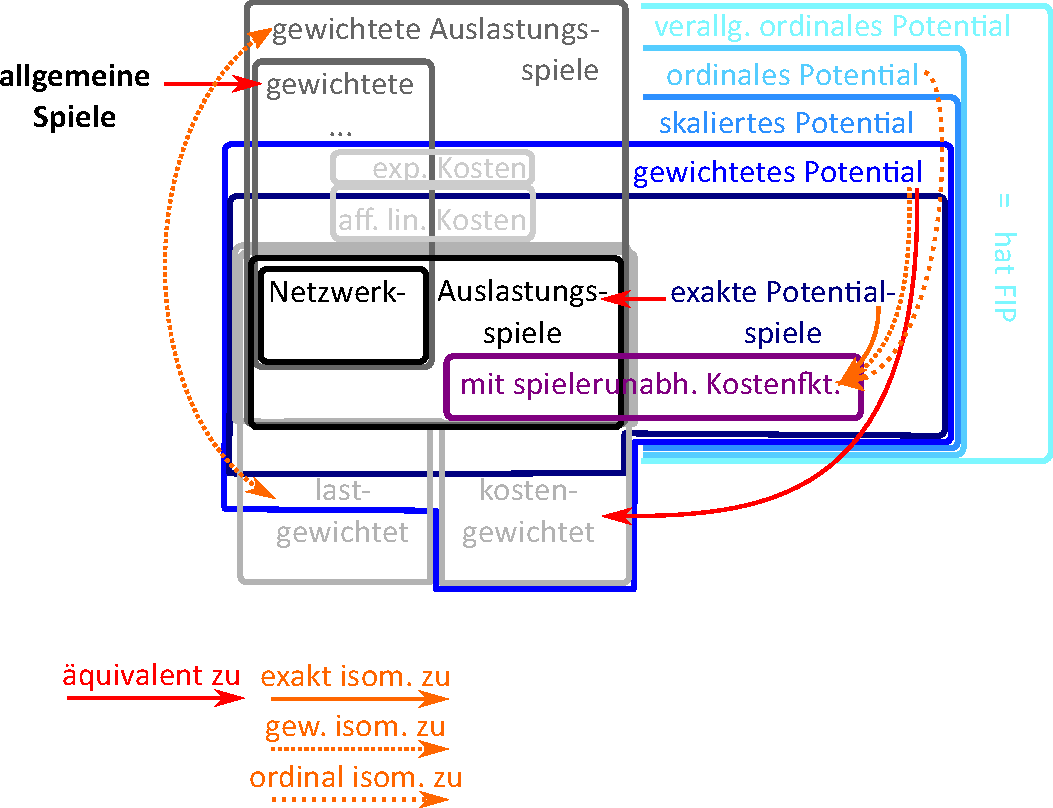
\includegraphics[width=.7\textwidth]{../Bilder/EulerDiagramm.pdf}
	\caption{Zusammenhänge zwischen den verschiedenen Spieleklassen für endliche Spiele}
\end{figure}